\documentclass[twocolumn, 11pt]{article} % MÅ defineres i ethvert dokument.
\usepackage{longtable}

\usepackage[utf8]{inputenc} %Tillater spesialteikn uten bruk av koding.
\usepackage[norsk]{babel} % Tillater norske teikn.
\usepackage[margin=1in]{geometry} % Definerer marger i dokumentet.
\usepackage{microtype} % Gjør det mer behagelig å lese dokumentet.
\usepackage{amsmath} % Tillater avansert formatering av matte.
\usepackage{amsfonts} % Tillater avanserte teikn, som R for reelle tall.
\usepackage[toc,page]{appendix} 
\usepackage{url}
\usepackage{graphicx} % Tillater mer avansert formatering av grafikk.
\usepackage{geometry} % Tillater enklere formatering av sidevisning.
\usepackage[colorlinks=true, pdfborder={0 0 0}]{hyperref} % Tillater hyperlenker {\href} som under. Colorlinks kan byttes til false hvis man ønsker linker i svart.
\usepackage[tableposition=top]{caption} % Tvinger tabelltekst til å dukke opp over alle tabeller.
\usepackage{graphicx}
\usepackage{float}
\graphicspath{ {./images/} }
\usepackage{listings}
\usepackage{color}
\definecolor{dkgreen}{rgb}{0,0.6,0}
\definecolor{gray}{rgb}{0.5,0.5,0.5}
\definecolor{mauve}{rgb}{0.58,0,0.82}
\lstset{frame=tb,
  language=Python,
  aboveskip=3mm,
  belowskip=3mm,
  showstringspaces=false,
  columns=flexible,
  basicstyle={\small\ttfamily},
  numbers=none,
  numberstyle=\tiny\color{gray},
  keywordstyle=\color{blue},
  commentstyle=\color{dkgreen},
  stringstyle=\color{mauve},
  breaklines=true,
  breakatwhitespace=true,
  tabsize=1
}
\begin{document}

\twocolumn[
  \begin{@twocolumnfalse}
\textbf{
  \title{Estimat av Plancks konstant ved hjelp av fotoelektrisk effekt}
  \author{Bård Tollef Pedersen og Erik Lykke Trier}
  \date{\today}
  \maketitle
} 
    \begin{abstract}
    \begin{large}
    \
    Formålet med denne rapporten er å estimere Plancks konstant ved hjelp av fotoelektriske effekten og minste kvadraters metode, samt sammenligne dette estimatet med den kjente verdien. Dette ble gjort ved å måle stoppotensialet til forskjellige bølgelengder, lage en regresjonslinje med disse dataene og multiplisere stigningstallet med elementær ladningen. Som  resultat ble det estimert at Plancks konstant er $6.537$ × $10^{-34}$ $\pm$ $4.623$ × $10^{-35}\textit{Js}$ som er unna den sanne verdien med en faktor på 1.34\%. 
    
    \end{large}
    \end{abstract}
  \end{@twocolumnfalse}     
  ]
\section{Innledning} 
La oss reise tilbake til begynnelsen av det 20. århundre, en tid da vitenskapelige pionerer utforsket verden på en helt ny måte. En av disse pionerene var Max Planck, som la grunnlaget for kvantemekanikk ved å introdusere begrepet 'kvant' og utvikle teorien om strålingsloven. I denne rapporten skal det estimeres en av de mest grunnleggende konstantene i kvantemekanikken - Plancks konstant. Dette blir gjort ved hjelp av den fotoelektriske effekten og minste kvadraters metode. Formålet er å estimere Plancks konstant, og sammenligne dette estimatet med den kjente verdien. 
    
\section{Teori og metoder}

\subsection{Fotoelektrisk effekt}
Fotoelektrisk effekt er en fysisk effekt som beskriver at når et materiale utsettes for lys med en bestemt energi, kan elektroner bli frigjort fra materialets overflate. Effekten ble oppdaget av den tyske fysikeren Heinrich Hertz i 1887, og fikk senere sin teoretiske forklaring av Albert Einstein i 1905.

Fotoelektrisk effekt skjer når et materiale utsettes for lys med en bølgelengde som har høyere energi enn materialets arbeidsfunksjon, en energi som kreves for å frigjøre elektroner fra materialet. Når lyset treffer materialet, overføres lys energien til elektronene, som fører til at elektronene blir frigjort fra materialets overflate.

Fotoelektrisk effekt har mange praktiske anvendelser, inkludert fotodetektorer i kamera, lysmålere i solarceller, og elektroniske enheter som benytter lys til å kontrollere strømmen av elektroner.

Fotoelektrisk effekt har også viktige implikasjoner for teoriene om lys og elektromagnetisme, da den gir en praktisk bekreftelse på at lys har både partikkel- og bølgeegenskaper\cite{Einstein}.

Fotoelektrisk effektapparatet som ble brukt i dette forsøket er AP-8209 fra Pasco.

\subsection{Bølgelengde og frekvens}
Bølgelengde refererer til avstanden mellom to nabotopper i en bølge, eller tilsvarende avstanden mellom to bølgetopper i en serie av bølger. Bølgelengde er en viktig egenskap ved bølger, inkludert elektromagnetiske bølger som lys og radio, og mekaniske bølger som lyd\cite{Bølgelengde}. 

Bølgelengden til en elektromagnetisk bølge bestemmes av frekvensen, og omvendt. For å endre fra bølgelengde til frekvens kan en bruke formel \eqref{lysfrekvensen}.

\begin{equation}
    f = \frac{c}{\lambda}
    \label{lysfrekvensen}
\end{equation}

I formel \eqref{lysfrekvensen}, er lysfart oppgitt som c og er en fysisk konstant. $\lambda$ er bølgelengde og formelen gir oss svaret i frekvens, \textit{f} oppgitt i \textit{Hz}.

Frekvens refererer til antall bølger som passerer et bestemt punkt i løpet av en gitt tid. Frekvens måles vanligvis i enheten Hertz (\textit{Hz}), som tilsvarer antall sykluser per sekund. Frekvensen til elektromagnetiske bølger bestemmer energien til bølgen, og høye frekvenser har høyere energi enn lave frekvenser\cite{Frekvens}.

\subsection{Elementærladning}
Elementærladning er den minste mengden elektrisk ladning som en partikkel kan ha, og den er representert av symbolet \textit{e}. Elementærladningen tilsvarer ladningen til et enkelt proton eller elektron. Den har en verdi på $1.602176 634$ × $10^{-19}$ Coulomb og spiller en sentral rolle i elektromagnetisme og kvantemekanikk \cite{elementærladning}.


\subsection{Minste kvadraters metode}
Minste kvadraters metode er en metode for å løse regresjonsproblemer, hvor målet er å finne den beste linjen som passer til et sett med observasjoner. Metoden fungerer ved å finne den linjen som har den minste summen av kvadrert avvik mellom observasjoner og den tilpassede linjen, hvor regresjonslinjen er gitt på følgende måte, formel \eqref{MinsteKvadraterLinje}.

\begin{equation}
    y_i = A +Bx_i
    \label{MinsteKvadraterLinje}
\end{equation}

I formel \eqref{MinsteKvadraterLinje} er y funksjonen til regresjonslinjen, A er konstantleddet og B er stigningstallen. 

For å regne ut av stigningstallen og konstantleddet til regresjonslinjen brukes formelene \eqref{MinsteKvadraterDelta}, \eqref{MinsteKvadraterA} og \eqref{MinsteKvadraterB}. Disse formelene er gitt med minste kvadraters metode.

\begin{equation}
    \Delta = N \Sigma x^2  - (\Sigma x)^2
    \label{MinsteKvadraterDelta}
\end{equation}

I formel \eqref{MinsteKvadraterDelta} er N antall målinger, $\Sigma x^2$ er summen av alle kvadrert x verdiene, og $(\Sigma x)^2$ er summen av alle x verdiene kvadrert.

\begin{equation}
    A = \frac{\Sigma y \Sigma x^2 - \Sigma x \Sigma xy}{\Delta}
    \label{MinsteKvadraterA}
\end{equation}

I formel \eqref{MinsteKvadraterA} er $\Sigma y$ summen av alle y verdiene, $\Sigma x^2$ er summen av alle kvadrerte x verdiene, $\Sigma x$ er summen av alle x verdiene og $\Sigma xy$ er summen av alle x og y verdiene multiplisert med sin korresponderende verdi. 

\begin{equation}
    B = \frac{N \Sigma xy  - \Sigma x \Sigma y}{\Delta}
    \label{MinsteKvadraterB}
\end{equation}

I formel \eqref{MinsteKvadraterB} er N antall målinger, $\Sigma xy$ er summen av alle x og y verdiene multiplisert med sin korresponderende verdi, $\Sigma x$ er summen av alle x verdiene og $\Sigma y$ summen av alle y verdiene. 

Minste kvadraters metode brukes ofte i statistikk, økonometri og andre områder for å analysere sammenhenger mellom variabler og for å forutsi verdier basert på tidligere observasjoner. Det er en enkel og effektiv metode for å løse regresjonsproblemer når antagelsene om en lineær sammenheng mellom variablene er oppfylt \cite{taylor1997error}. 

Som alt annet er det en standardfeil ved å regne på minste kvadraters metode. Denne standardfeilen er gitt ved formel \eqref{UsikkerhetY}, \eqref{UsikkerhetA} og \eqref{UsikkerhetB}.

\begin{equation}
    \sigma y = \Sigma \sqrt{\frac{1}{N-2}*(y-A-B*x)^2}
    \label{UsikkerhetY}
\end{equation}

I formel \eqref{UsikkerhetY} er N antall målinger. A, B, y og x er verdiene fra funksjonen for regresjonslinjen, gitt med formel \eqref{MinsteKvadraterLinje}.

\begin{equation}
    \sigma A = \sigma y * \sqrt{\frac{\sum x^2}{\Delta}}
    \label{UsikkerhetA}
\end{equation}

I formel \eqref{UsikkerhetA} er $\sigma y$ standardfeilen gitt ved formel \eqref{UsikkerhetY}. $\Delta$ er gitt ved formel \eqref{MinsteKvadraterDelta} og $\sum x^2$ er summen av alle kvadrerte x verdiene.

\begin{equation}
    \sigma B = \sigma y * \sqrt{\frac{N}{\Delta}}
    \label{UsikkerhetB}
\end{equation}

I formel \eqref{UsikkerhetB} er $\sigma y$ standardfeilen gitt ved formel \eqref{UsikkerhetY}. $\Delta$ er gitt ved formel \eqref{MinsteKvadraterDelta} og N er antall målinger.


\subsection{Plancks konstant}
Plancks konstant, symbolisert med \textit{h}, er en av de mest grunnleggende størrelsene i fysikken. Konstanten ble oppdaget av den tyske fysikeren Max Planck i 1900, og det var en av de første indikasjonene på at det var kvantemekanikken som regjerte i mikroskopiske områder. Plancks konstant har en stor betydning for mange områder i fysikken, inkludert elektromagnetisme, kjernefysikk, og spektroskopi.

Verdien av Plancks konstant er fastsatt til $6.62607015$ × $10^{-34}$ joule-sekunder, og den brukes ofte sammen med den elektromagnetiske konstanten og lysets hastighet til å beskrive relasjonen mellom energi og frekvens i elektromagnetisk stråling.

Plancks konstant er en av de mest nøyaktige konstantene i fysikken, og det er en av de fire fundamentale naturkonstantene som bestemmer hvordan universet fungerer\cite{Planckskonstant}.


Ved hjelp av minste kvadraters metode kan en estimere Plancks konstant. Dette estimatet baserer seg på frekvens og fotoelektrisk effekt. Der stigningen i regresjonslinen fra minste kvadraters metode gir et estimat for Plancks konstant ved hjelp av formel \eqref{b_equ} og \eqref{sigma_planck}. Hvor formel \eqref{sigma_planck} er standardfeilen for Plancks konstant. Formel \eqref{b_equ} og \eqref{sigma_planck} er hentet fra oppgaveteksten \cite{oppgavetekst}.


\begin{equation}
    B = \frac{h}{e}
    \label{b_equ}
\end{equation}

I formel \eqref{b_equ}, er \textit{h} Plancks konstant og \textit{e} er elementærladningen. Dette gir stigningstallet til regresjonslinen, \textit{B}.

\begin{equation}
    \delta h = e \delta B
    \label{sigma_planck}
\end{equation}

I formel \eqref{sigma_planck}, er $\delta \textit{B}$ er standardfeilen til stigningstallet til regresjonslinen og \textit{e} er elementærladning. Dette gir standardfeilen til Plancks konstant, $\delta \textit{h}$.


\section{Resultater}

Resultatet er oppgitt i tabellen under, tabell \ref{tabell_volt}. Her kan en se de forskjellige filtrene brukt for å oppnå de forskjellige bølgelengdene, oppgitt i \textit{nm}. En kan også se de relative stoppotensialene til de representative bølgelengdene, oppgitt i \textit{V}.

\begin{table}[h]
\caption{Viser resultater fra målingene med fotoelektrisk
effekt.}
\begin{tabular}{|l|l|ll}
\cline{1-2}
Bølgelengde(\textit{nm})  &   Volt(\textit{V})   &  &  \\ \cline{1-2}
365  &   1.845   &  &  \\ \cline{1-2}
405  &   1.416   &  &  \\ \cline{1-2}
436  &   1.286   &  &  \\ \cline{1-2}
546  &   0.708   &  &  \\ \cline{1-2}
577  &   0.580   &  &  \\ \cline{1-2}

\end{tabular}
\label{tabell_volt}
\end{table}


Fra tabell \ref{tabell_volt} og ved hjelp av minste kvadraters metode, gitt med formlene \eqref{MinsteKvadraterLinje},\eqref{MinsteKvadraterDelta}, \eqref{MinsteKvadraterA}, \eqref{MinsteKvadraterB} får vi verdiene oppgitt i tabell \ref{minste_resultat}. Her kan en se verdiene til A, B og formelen for regresjonslinjen, samt usikkerheten for de tilsvarende verdiene. Usikkerhetene er beregnet med formel \eqref{UsikkerhetY}, \eqref{UsikkerhetA} og \eqref{UsikkerhetB}.

%$A=-1.5404691118579386$,
%$B=4.080197445028516e-15$ og
%$y=-1.540 + 4.080e-15*x$

\begin{table}[h]
\caption{Viser verdiene for regresjonslinja ved minste kvadraters metode.}
\begin{tabular}{|l|l|l|ll}
\cline{1-3}
  & Verdi                                       & Usikkerhet &  &  \\ \cline{1-3}
A & $-1.540$                                      & $0.194$  &  &  \\ \cline{1-3}
B & $4.080$ × $10^{-15}$                              & $2.885$ × $10^{-16}$  &  &  \\ \cline{1-3}
y & $-1.540+4.080$×$10^{-15}$                      & $0.0737$ &  &  \\ \cline{1-3}
\end{tabular}
\label{minste_resultat}
\end{table}

Regresjonslinjen fra tabell \ref{minste_resultat} kan en se plottet i figur \ref{plot_plack}. Her kan en se de blå punktene som rådata, den grønne linjen som regresjonslinjen fra tabell \ref{minste_resultat} og den røde linjen som regresjonslinjen ved bruk av den sanne Plancks konstant, hvor konstanten er hentet fra \cite{Planckskonstant}.

\begin{figure}[H]
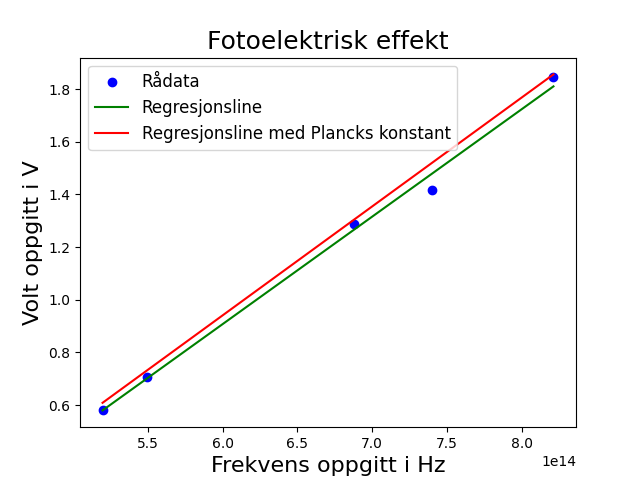
\includegraphics[width=0.49\textwidth]{Images/lab4.png}
\caption{Plott av Fotoelektrisk effekt som viser  stoppotensialet som funksjon av frekvens, hvor stigningstallet multiplisert med elementær ladning er et estimatet på Plancks konstant.}
\label{plot_plack}
\end{figure}

Ved hjelp av tabell \ref{minste_resultat} og formel \eqref{b_equ} får vi et estimat av Plancks konstant med en verdi på $6.537$ × $10^{-34}\textit{Js}$. Med samme tabell og formel \ref{sigma_planck} får vi en usikkerhet til denne konstanten på $\pm$ $4.623$ × $10^{-35}\textit{Js}$.

Koden brukt for å regne ut Plancks konstant, samt plotte figur \ref{plot_plack} kan sees i vedlegg \ref{Python}. Rådata kan en finne i vedlegg \ref{RådataVedlegg}.


\section{Diskusjon}

Fra figur \ref{plot_plack} kan en se at regresjonslinjen fra forsøket og regresjonslinjen plottet med den sanne Plancks konstant er relativt like. En kan se at regresjonslinjen plottet med den sanne Plancks konstant er litt høyre. En kan også se at den har en større stigning. Dette gir oss en indikasjon på hvordan den sanne Plancks konstant er relativt til den estimerte. Her kan en se at den sanne verdien er litt større enn estimatet. Hadde det blitt tatt fler repetisjoner av forsøket kunne regresjonslinjene vært enda mer parallelle. Flere punkter hadde plottet seg jevnt rundt den sanne verdien sin regresjonslinje og det ville blitt ett bedre estimat. Ulempen med flere forsøk er at det gir større mulighet for uteliggere som kunne påvirket negativt på regresjonslinjen og estimatet.
 
Fra manualen til apparatet AP-8209 ser en at ampere målingen gir en usikkerhet på $\pm$ 0.2\% etter 20 min oppvarming, og en usikkerhet på volt avlesning på $\leq$ 0.1\%. Dette er lite i forhold til estimatet som har en usikkerhet på $\pm$ $4.623$ × $10^{-35}\textit{Js}$. Manualen sier også at målingsfeilen ved dette forsøket ofte er $\pm 3\%$. Dette vil si at alt innenfor den sanne verdien $\pm 3\%$ er akseptable verdier med dette måle apparatet \cite{AP-8209}.

De fleste feilkildene ved dette forsøket er ved apparatet. Her kan blant annet dårlig kalibrering føre til feil. Dårlig kalibrering kan både føre til at resultatene er mer ujevne, men også at resultatene blir for lave. Ved jevne men lave resultater vil stigningen fortsatt være et estimat på Plancks konstant, så lenge alle verdiene er lave med samme faktor. Derimot når kalibreringen fører til ujevne resultater vil regresjonslinjen bli unøyaktig, spesielt ved så få målinger vil selv en dårlig måling ha et stort innspill på resultatet. 

En annen feilkilde fra apparatet kan være å ikke la den varme seg opp lengde nok. I manualen står det at den skal varmes opp i 20 minutter før den skal kalibreres. Dette er for at lampen skal bli varm nok. Å starte forsøket for tidlig vil gjøre at det er stor forskjell mellom første og siste måling, der første vil være unøyaktig, men riktig kalibrert, mens siste vil være nøyaktig men feil kalibrert. Dette kan gjøre at regresjonslinen får en drastisk stignings endring i forhold til hva som er forventet.
Apparatet blir også påvirket av romtemperaturen. Så dette kan være en faktor til hvorfor en ikke får perfekt resultat. Dette er en faktor ettersom romtemperaturen påvirker stoffets fotoelektriske effekt. Dette vil gjøre at en får lavere eller høyrer stoppotensial, men så lenge romtemperaturen er jevn vil også resultatet være jevnt og det vil være en liten feilkilde.

Det kan også være feil i Python koden som er brukt for å regne ut både regresjonslinjen og Plancks konstant.

\section{Konklusjon}

Estimatet på Plancks konstant ble $6.537$ × $10^{-34}$ $\pm$ $4.623$ × $10^{-35}\textit{Js}$. Ifølge SNL er Plancks konstant $6.62607015$ × $10^{-34}\textit{Js}$, som vil si at den sanne verdien er vel innenfor den estimerte verdien med standardfeilene\cite{Planckskonstant}. I tillegg sier manualen ti' AP-8209 at målingsfeil ved dette forsøket ofte er på 3 prosent, estimatet fra denne rapporten har en målingsfeil på 1,34 prosent. Så resultatet er et godt estimat på Plancks konstant.

 

\bibliographystyle{plain}
\bibliography{sources4.bib}
\clearpage

\onecolumn
\newpage
\appendix
\section{Vedlegg A}
\label{Python}

\begin{lstlisting}
import math
import matplotlib.pyplot as plt  # Import packages for script to run

y = [1.845, 1.416, 1.286, 0.708, 0.580]  # Data that will be the y-values in Volt
list_of_nm = [365, 405, 436, 546, 577]  # Data that will be the x-values in nm
speed_of_light = 299792458  # The speed of light in m/s
x = []
for i in range(len(list_of_nm)):
    temp = speed_of_light / (list_of_nm[i] * (10 ** (-9)))  # Turn wavelength to frequency in Hz
    x.append(temp)

"""
Create variables and calculate A and B.
"""
x_sum = 0
x_kvadrat_sum = 0
y_sum = 0
xy_sum = 0
N = len(x)
sigma_y = 0
for i in range(len(x)):
    x_sum += x[i]
    xy_sum += x[i] * y[i]
    y_sum += y[i]
    x_kvadrat_sum += x[i] ** 2

delta = N * x_kvadrat_sum - x_sum ** 2
A = (y_sum * x_kvadrat_sum - x_sum * xy_sum) / delta
B = (N * xy_sum - x_sum * y_sum) / delta

"""
Calculate all the standard error.
"""
for i in range(len(x)):
    sigma_y += math.sqrt((1 / (N - 2)) * (y[i] - A - B * x[i]) ** 2)

sigma_A = sigma_y * math.sqrt(x_kvadrat_sum / delta)
sigma_B = sigma_y * math.sqrt(N / delta)

print('A:', A, '  B: ', B, '\n', 'Standard error to A:', sigma_A,
      'Standard error to b:', sigma_B, 'Standard error to y:', sigma_y)

"""
Calculate Placks constant.
"""

e = 1.60217656535 * (10 ** (-19))  # elementary charge in Colomb
h = 6.62607015 * (10**-34)  # The true value of Placks constant

print('Placks constant: ', B*e, 'Standard error to Placks constant: ', sigma_B * e)
print('Accuracy in percentage', (100 - ((B*e)/h) * 100))


"""
For plotting the line and data.
"""
list_plot_y = []
for i in range(len(x)):
    y_1 = A + B*x[i]
    list_plot_y.append(y_1)

plt.scatter(x, y, color='blue')
plt.plot(x, list_plot_y, color='green')

B = h/e
list_plot_y = []
for i in range(len(x)):
    y_1 = A + B*x[i]
    list_plot_y.append(y_1)

plt.plot(x, list_plot_y, color='red')
plt.title('Fotoelektrisk effekt', fontsize=18)
plt.xlabel('Frekvens oppgitt i Hz', fontsize=16)
plt.ylabel('Volt oppgitt i V', fontsize=16)
plt.legend(['Rådata', 'Regresjonsline', 'Regresjonsline med Plancks konstant'], fontsize=12)
plt.savefig('lab4.png')

\end{lstlisting}

\newpage
\section{Vedlegg B}
\label{RådataVedlegg}

\begin{longtable}{ll}

365 nm      & -1.845 V\\
405 nm      & -1.416 V\\
436 nm      & -1.286 V\\
546 nm      & -0.708 V\\
577 nm      & -0.580 V\\
            &       
\end{longtable}

\end{document}